\documentclass[tikz,border=6pt]{standalone}
% Shared style for MultiMM figures (white background, logo palette)
\usepackage{tikz,pgfplots,amsmath}
\pgfplotsset{compat=1.16}
\usetikzlibrary{arrows.meta,calc,decorations.pathreplacing,positioning,backgrounds}
\definecolor{indigo}{HTML}{3B37A0}
\definecolor{violet}{HTML}{6A3AA8}
\definecolor{crimson}{HTML}{B5406C}
\definecolor{gold}{HTML}{E9A62C}
\definecolor{golddark}{HTML}{B9791A}
\definecolor{grey}{HTML}{8A8AA0}
\definecolor{lightgrey}{HTML}{E4E4EE}
\tikzset{
  bead/.style={circle,draw=#1!80!black,fill=#1!35,line width=0.5pt,minimum size=9pt,inner sep=0pt},
  bead/.default=indigo,
  lab/.style={font=\small},
}
\pgfplotsset{
  every axis/.append style={
    width=9.5cm,height=6.3cm,axis lines=left,line width=0.5pt,
    grid=major,grid style={draw=lightgrey,line width=0.3pt},
    tick label style={font=\small},label style={font=\normalsize},
    legend style={font=\footnotesize,draw=none,fill=white,fill opacity=0.8,text opacity=1},
    legend cell align=left,
  },
  every axis plot/.append style={line width=1.2pt,smooth},
}

\begin{document}
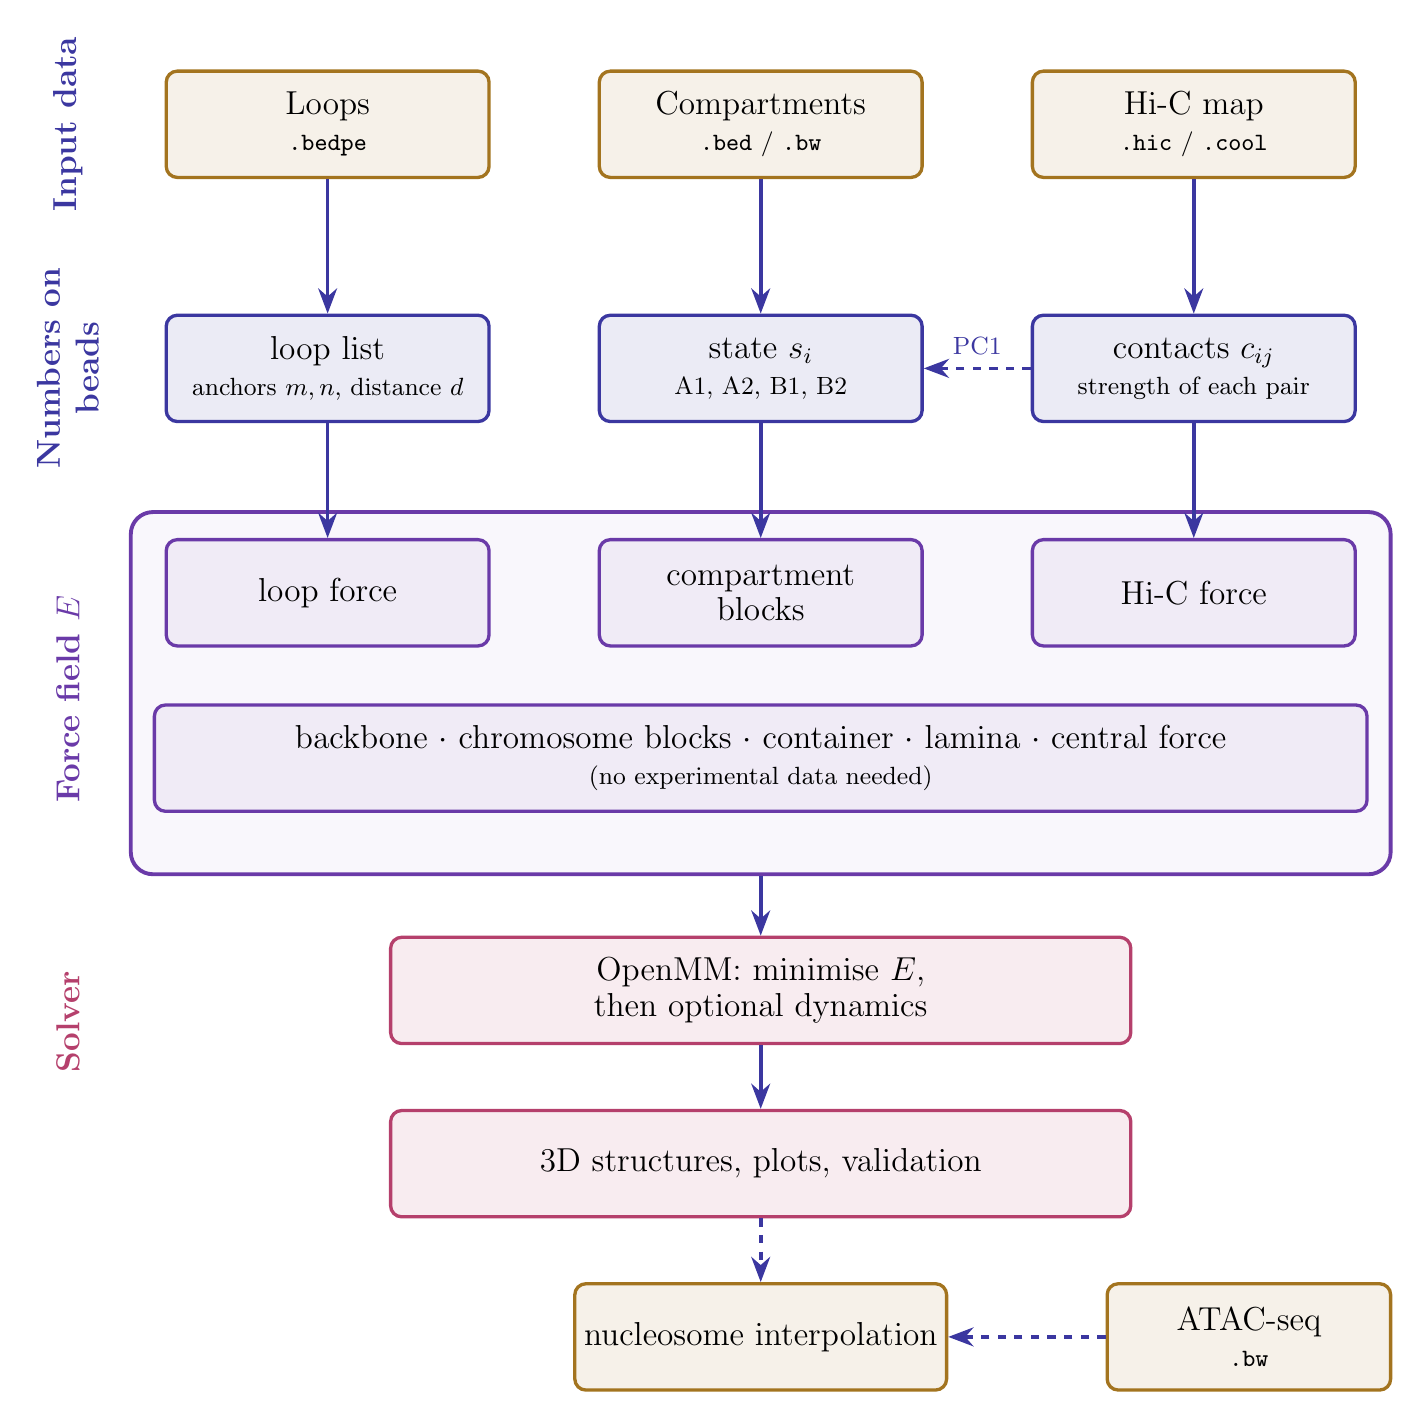
\begin{tikzpicture}[
  box/.style={draw=#1,fill=#1!10,rounded corners=4pt,line width=1.2pt,minimum width=4.1cm,minimum height=1.35cm,align=center,font=\large},
  box/.default=indigo,
  wide/.style={draw=#1,fill=#1!10,rounded corners=4pt,line width=1.2pt,minimum height=1.35cm,align=center,font=\large},
  arr/.style={-{Stealth[length=3.2mm]},line width=1.3pt,indigo},
  head/.style={font=\large\bfseries,text=#1}, head/.default=indigo]
% 1 input data
\node[head,rotate=90] at (-8.8,0) {Input data};
\node[box=gold!70!black] (lp) at (-5.5,0) {Loops\\[-1pt]{\small \texttt{.bedpe}}};
\node[box=gold!70!black] (cp) at (0,0)   {Compartments\\[-1pt]{\small \texttt{.bed} / \texttt{.bw}}};
\node[box=gold!70!black] (hc) at (5.5,0) {Hi-C map\\[-1pt]{\small \texttt{.hic} / \texttt{.cool}}};
% 2 per-bead quantities
\node[head,rotate=90,align=center] at (-8.8,-3.1) {Numbers on\\beads};
\node[box] (ll) at (-5.5,-3.1) {loop list\\[-1pt]{\small anchors $m,n$, distance $d$}};
\node[box] (st) at (0,-3.1)    {state $s_i$\\[-1pt]{\small A1, A2, B1, B2}};
\node[box] (cc) at (5.5,-3.1)  {contacts $c_{ij}$\\[-1pt]{\small strength of each pair}};
\draw[arr] (lp)--(ll); \draw[arr] (cp)--(st); \draw[arr] (hc)--(cc);
\draw[arr,dashed] (cc.west)--(st.east) node[midway,above=1pt,font=\small,text=indigo] {PC1};
% 3 force field
\node[head=violet,rotate=90] at (-8.8,-7.3) {Force field $E$};
\begin{scope}[on background layer]
\node[draw=violet,fill=violet!4,rounded corners=8pt,line width=1.4pt,minimum width=16.0cm,minimum height=4.6cm,anchor=north] (ff) at (0,-4.9) {};
\end{scope}
\node[box=violet] (lf) at (-5.5,-5.95) {loop force};
\node[box=violet] (cb) at (0,-5.95)    {compartment\\[-1pt]blocks};
\node[box=violet] (hf) at (5.5,-5.95)  {Hi-C force};
\node[wide=violet,minimum width=15.4cm] (bb) at (0,-8.05) {backbone $\cdot$ chromosome blocks $\cdot$ container $\cdot$ lamina $\cdot$ central force\\[-1pt]{\small (no experimental data needed)}};
\draw[arr] (ll)--(lf); \draw[arr] (st)--(cb); \draw[arr] (cc)--(hf);
% 4 OpenMM
\node[head=crimson,rotate=90] at (-8.8,-11.4) {Solver};
\node[box=crimson,minimum width=9.4cm] (omm) at (0,-11.0) {OpenMM: minimise $E$,\\[-1pt]then optional dynamics};
\draw[arr] (ff.south)--(omm.north);
% 5 outputs
\node[box=crimson,minimum width=9.4cm] (out) at (0,-13.2) {3D structures, plots, validation};
\draw[arr] (omm)--(out);
\node[box=gold!70!black,minimum width=4.6cm] (nuc) at (0,-15.4) {nucleosome interpolation};
\node[box=gold!70!black,minimum width=3.6cm] (at) at (6.2,-15.4) {ATAC-seq\\[-1pt]{\small \texttt{.bw}}};
\draw[arr,dashed] (out)--(nuc);
\draw[arr,dashed] (at)--(nuc);
\end{tikzpicture}
\end{document}
